% UML Class Diagram: Comparison across branches
% Compile: pdflatex uml-comparison.tex

\documentclass[tikz,border=10pt]{standalone}
\usepackage[T1]{fontenc}
\usepackage{tikz}
\usetikzlibrary{positioning,shapes,arrows,calc}

\begin{document}

% Branch 09-00: Monolithic
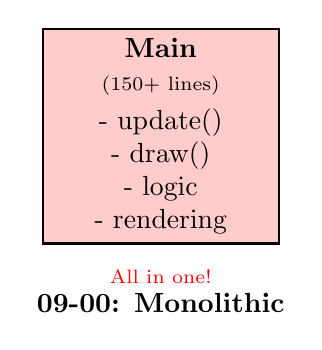
\begin{tikzpicture}[
    class/.style={rectangle, draw=black, thick, minimum width=3cm, minimum height=1cm, align=center},
    problem/.style={fill=red!20},
    node distance=2cm
]
    \node[class, problem] (main00) {
        \textbf{Main} \\
        \scriptsize (150+ lines) \\[2pt]
        - update() \\
        - draw() \\
        - logic \\
        - rendering
    };

    \node[below=0.5cm of main00] {\textbf{09-00: Monolithic}};
    \node[below=0.2cm of main00, text=red] {\scriptsize All in one!};
\end{tikzpicture}

\vspace{1cm}

% Branch 09-01: Game Loop
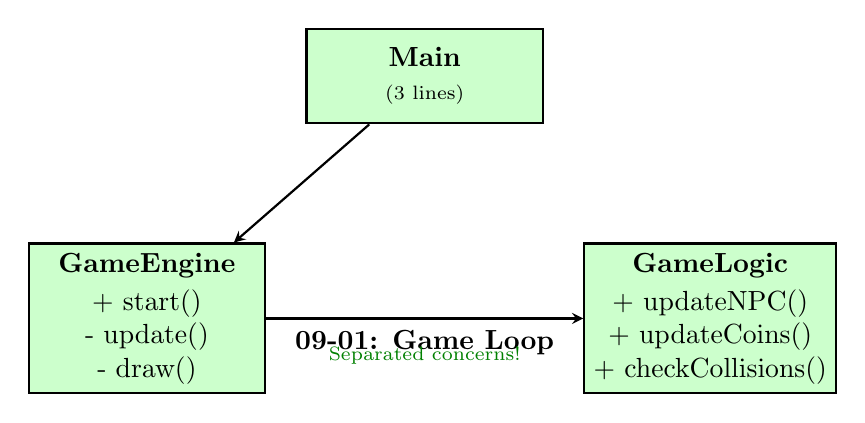
\begin{tikzpicture}[
    class/.style={rectangle, draw=black, thick, minimum width=3cm, minimum height=1.2cm, align=center},
    solution/.style={fill=green!20},
    arrow/.style={->,>=stealth,thick}
]
    \node[class, solution] (main01) {
        \textbf{Main} \\
        \scriptsize (3 lines)
    };

    \node[class, solution, below left=1.5cm and 0.5cm of main01] (engine01) {
        \textbf{GameEngine} \\[2pt]
        + start() \\
        - update() \\
        - draw()
    };

    \node[class, solution, below right=1.5cm and 0.5cm of main01] (logic01) {
        \textbf{GameLogic} \\[2pt]
        + updateNPC() \\
        + updateCoins() \\
        + checkCollisions()
    };

    \draw[arrow] (main01) -- (engine01);
    \draw[arrow] (engine01) -- (logic01);

    \node[below=2.5cm of main01] {\textbf{09-01: Game Loop}};
    \node[below=2.7cm of main01, text=green!50!black] {\scriptsize Separated concerns!};
\end{tikzpicture}

\vspace{1cm}

% Branch 09-02: Without Singleton
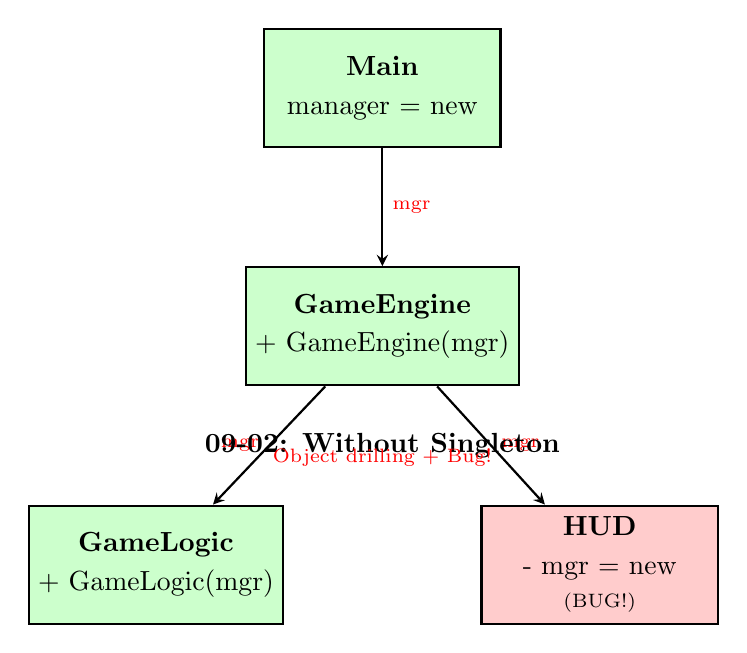
\begin{tikzpicture}[
    class/.style={rectangle, draw=black, thick, minimum width=3cm, minimum height=1.5cm, align=center},
    problem/.style={fill=red!20},
    solution/.style={fill=green!20},
    arrow/.style={->,>=stealth,thick},
    param/.style={red,font=\scriptsize}
]
    \node[class, solution] (main02) {
        \textbf{Main} \\[2pt]
        manager = new
    };

    \node[class, solution, below=1.5cm of main02] (engine02) {
        \textbf{GameEngine} \\[2pt]
        + GameEngine(mgr)
    };

    \node[class, solution, below left=1.5cm and -0.5cm of engine02] (logic02) {
        \textbf{GameLogic} \\[2pt]
        + GameLogic(mgr)
    };

    \node[class, problem, below right=1.5cm and -0.5cm of engine02] (hud02) {
        \textbf{HUD} \\[2pt]
        - mgr = new \\
        \scriptsize (BUG!)
    };

    \draw[arrow] (main02) -- node[right,param] {mgr} (engine02);
    \draw[arrow] (engine02) -- node[left,param] {mgr} (logic02);
    \draw[arrow] (engine02) -- node[right,param] {mgr} (hud02);

    \node[below=3.5cm of main02] {\textbf{09-02: Without Singleton}};
    \node[below=3.7cm of main02, text=red] {\scriptsize Object drilling + Bug!};
\end{tikzpicture}

\vspace{1cm}

% Branch 09-03: With Singleton
\begin{tikzpicture}[
    class/.style={rectangle, draw=black, thick, minimum width=3cm, minimum height=1.5cm, align=center},
    solution/.style={fill=green!20},
    singleton/.style={fill=blue!20},
    arrow/.style={->,>=stealth,thick},
    dashedarrow/.style={->,>=stealth,thick,densely dashed,blue}
]
    \node[class, solution] (main03) {
        \textbf{Main} \\
        \scriptsize (3 lines)
    };

    \node[class, solution, below=1.5cm of main03] (engine03) {
        \textbf{GameEngine} \\[2pt]
        + GameEngine()
    };

    \node[class, solution, below left=1.5cm and -0.5cm of engine03] (logic03) {
        \textbf{GameLogic} \\[2pt]
        + GameLogic()
    };

    \node[class, solution, below right=1.5cm and -0.5cm of engine03] (hud03) {
        \textbf{HUD} \\[2pt]
        + HUD()
    };

    \node[class, singleton, right=3cm of engine03] (mgr03) {
        \textbf{GameManager} \\
        \scriptsize «singleton» \\[2pt]
        - instance \\
        + getInstance()
    };

    \draw[arrow] (main03) -- (engine03);
    \draw[arrow] (engine03) -- (logic03);
    \draw[arrow] (engine03) -- (hud03);

    \draw[dashedarrow] (logic03) -- (mgr03) node[midway,above,sloped,font=\scriptsize,blue] {getInstance()};
    \draw[dashedarrow] (hud03) -- (mgr03) node[midway,below,sloped,font=\scriptsize,blue] {getInstance()};

    \node[below=3.5cm of main03] {\textbf{09-03: With Singleton}};
    \node[below=3.7cm of main03, text=green!50!black] {\scriptsize Clean + Fixed!};
\end{tikzpicture}

\end{document}
